\documentclass[a4paper, 12pt]{article}
\usepackage[top=1cm, bottom=2.1cm, left=2cm, right=2cm]{geometry}
\usepackage[utf8]{inputenc}
\usepackage{graphicx, caption}
\usepackage{float}
\usepackage{amsmath, amsfonts, amssymb, esint}
\usepackage{hyperref}
\usepackage{multicol}
\usepackage{color}
\usepackage{wallpaper}
\usepackage{array}

\CenterWallPaper{1}{./img/background.png}

\hypersetup{
    colorlinks=true,
    linkcolor=blue,
    filecolor=magenta,      
    urlcolor=cyan,
}

\definecolor{red}{rgb}{1,0,0}
\newcommand{\red}[1]{\textcolor{red}{#1}}

\newcolumntype{M}[1]{>{\centering\arraybackslash}m{#1}}

\begin{document}
    \begin{figure}
        \centering
        \href{https://ligaolimpicadeastronomia.com.br/}{
\includegraphics[scale=0.6]{./img/logos.png}}
    \end{figure}
    \begin{center}
        \begin{large}
            \textbf{Simulado -- Intensivão para a OBA}
            \linebreak \red{Gabarito}
        \end{large}
        \end{center}
    \begin{flushright}
        Material elaborado por \textbf{Iago Mendes}
    \end{flushright}

    \begin{flushleft} \begin{itemize}
        \item \textbf{Questão 1) (1 ponto)} Todas as civilizações da Antiguidade que nos deixaram registros astronômicos observaram que, além das estrelas que pareciam fixas umas em relação às outras, existiam cinco pontos luminosos que passeavam por entre as estrelas, os planetas visíveis a olho nu: Mercúrio, Vênus, Marte, Júpiter e Saturno. Os demais planetas não eram conhecidos nesta época, pois não havia telescópios. A partir da invenção do telescópio – utilizado pela primeira vez por Galileu Galilei para estudar o céu – foram identificados os demais planetas, além de diversos outros corpos celestes não observáveis a olho nu, como satélites planetários, um grande número de asteroides e cometas de baixa luminosidade. Uma primeira estrutura foi identificada no início do século XIX, o Cinturão de Asteroides, cujos componentes foram descobertos em sequência à descoberta do maior deles, Ceres (descoberto em 1801 por Giuseppe Piazzi), que, com seus 950 km de diâmetro, apesar de esférico, era pequeno demais para ser considerado um planeta. Além disso, vários outros corpos bem menores, basicamente rochosos, foram observados tendo órbitas entre Marte e Júpiter. Hoje, os astrônomos julgam que Júpiter teria impedido a formação de um planeta entre ele e Marte dando origem a este cinturão. É importante mencionar que a formação dos corpos do Sistema Solar (Sol, planetas e demais corpos) deu-se por aglutinação de corpos menores ao longo de alguns poucos milhões de anos, partindo da condensação de uma nuvem de gás e poeira primordial. Os astrônomos atualmente também concordam que existem duas outras regiões de corpos menores no Sistema Solar e até acham que estes corpos estão lá porque foram expulsos quando os planetas já estavam formados. A primeira destas estruturas, que começa logo depois da órbita de Netuno, é o assim chamado Cinturão de Kuiper, cujos corpos estão espalhados em órbitas próximas ao plano das órbitas dos planetas. À medida que nos afastamos mais ainda do Sol, as órbitas dos corpos menores vão se espalhando por uma região cada vez mais extensa, até que a cerca de 0,5 ano luz do Sol, indo até 1 ano luz, as órbitas estão tão espalhadas que encontramos corpos com órbitas em qualquer ângulo em relação ao plano das órbitas dos planetas. Esta estrutura que envolve esfericamente todo o Sistema Solar, a uma grande distância dos planetas, é chamada de Nuvem de Oort. Para se ter uma ideia do quão longe significa 0,5 ano luz de distância, Netuno está a apenas cerca de 4 horas (!) luz e Plutão a pouco mais de 5 horas luz do Sol. Os corpos constituintes do Cinturão de Kuiper e da Nuvem de Oort são, em sua grande maioria, formados de constituintes mais leves, como água, metano e, em menor quantidade elementos rochosos, ou seja, o que é chamado de gelo sujo. Acredita-se, inclusive, que a origem dos oceanos terrestres teria sido um bombardeamento por cometas. Na verdade, Jan Hendrik Oorte Gerard Peter Kuiper ao proporem, no início da década de 50 do século passado, as estruturas que terminaram por receber seus nomes, estavam pensando nesta outra classe de corpos menores, os cometas, já então com grande número de ocorrências registradas e estudadas à época. Assim, cometas de período da ordem do Cometa Halley, isto é de ``curto período'', com órbitas próximas ao plano da órbita dos planetas, seriam lançados em direção ao Sol por perturbações gravitacionais nos corpos do Cinturão de Kuiper e os de longo período (às vezes de milhares de anos), como possuíam órbitas em qualquer plano, viriam da Nuvem de Oort. Mas foi somente a partir da década de 1990, com o telescópio espacial Hubble e uma nova geração de grandes telescópios, que muitos corpos menores, muito além da órbita de Netuno, foram identificados. Dentre os maiores objetos estão: Sedna, descoberto em 2002, Quaoar e 2004DW, descobertos em 2004 e, o maior de todos, Eris, maior inclusive que Plutão, descoberto em 2005. Assim, Plutão, com sua órbita um pouco fora do plano da órbita dos planetas, com seu tamanho diminuto, com sua composição mais próxima da de um cometa do que de um planeta rochoso e não sendo o único corpo a completar três voltas em torno do Sol enquanto Netuno completa duas, ficou cada vez mais diferente de corpos grandes e rochosos como Mercúrio, Vênus, Terra, Marte e dos gigantes gasosos, como Júpiter, Saturno, Urano e Netuno. Tais novas descobertas e a descoberta de planetas extra-solares (como será discutido na questão 5), colocaram como inadiável a discussão, pela União Astronômica Internacional (em inglês, IAU), sobre o que é de fato um planeta. O resultado foi amplamente divulgado no ano passado: Plutão deixou de ser classificado como planeta e junto com Ceres e Eris recebeu a classificação de ``planeta anão'', que não é um planeta, sendo classificado como um objeto que seria um planeta se fosse dominante e único em sua órbita de translação.
            \begin{itemize}
                \item \textbf{Pergunta 1a) (0,3 ponto) (0,05 cada acerto)} Nas colunas abaixo, marque as propriedades de cada astro.
                    \begin{center} \begin{tabular}
                    {
                        |M{0.15\textwidth}|M{0.15\textwidth}|M{0.15\textwidth}|M{0.15\textwidth}|M{0.15\textwidth}|
                    }
                        \hline
                        $\quad$ & Orbita o Sol diretamente. & Possui forma quase esférica. & É o astro dominante em sua órbita. & É um planeta. \\ \hline
                        Vênus & $\red{X}$ & $\red{X}$ & $\red{X}$ & $\red{X}$ \\ \hline
                        Plutão & $\red{X}$ & $\red{X}$ & $\quad$ & $\quad$ \\ \hline
                        Ceres & $\red{X}$ & $\red{X}$ & $\quad$ & $\quad$ \\ \hline
                        Lua & $\quad$ & $\red{X}$ & $\red{X}$ & $\quad$ \\ \hline
                        Ganimedes & $\quad$ & $\red{X}$ & $\red{X}$ & $\quad$ \\ \hline
                        Cometa Halley & $\red{X}$ & $\quad$ & $\quad$ & $\quad$ \\ \hline
                    \end{tabular} \end{center}
                \item \textbf{Pergunta 1b) (0,35 ponto)} Somente corpos grandes são aproximadamente esféricos porque neles um fator dominante de formação é grande o suficiente para atingir tal formato. Qual é esse fator?
                    \begin{itemize}
                        \item[$(\red{X})$] Gravidade
                        \item[$(\quad)$] Densidade
                        \item[$(\quad)$] Volume
                        \item[$(\quad)$] Albedo
                    \end{itemize}
                \item \textbf{Pergunta 1c) (0,35 ponto)} O cometa McNaught foi visível em janeiro de 2007 primeiro no Hemisfério Norte, com baixa luminosidade, e depois, muito mais brilhante, no Hemisfério Sul. De onde esse cometa se originou? Dica: para que isso seja possível, a órbita do cometa não pode ser paralela às órbitas no Sistema Solar.
                    \begin{itemize}
                        \item[$(\quad)$] Cinturão de Kuiper
                        \item[$(\quad)$] Cinturão de Asteroides
                        \item[$(\red{X})$] Nuvem de Oort
                        \item[$(\quad)$] Centro galáctico
                    \end{itemize}
            \end{itemize}

        \item \textbf{Questão 2) (1 ponto)} O eclipse total do Sol é impressionante, pois o céu fica escuro, podemos ver as estrelas, planetas e também a fabulosa ``coroa sola''. Contudo, infelizmente, o eclipse solar total tem curta duração, no máximo de alguns minutos. O da Lua, por outro lado, pode durar horas. Vejamos o porquê disso. \linebreak \linebreak Abaixo está um esquema mostrando o Sol, de raio $R_S$, a Terra, de raio $R_T$, e metade do ``cone de sombra'' da Terra. Sabemos que $R_S = 109 \cdot R_T$ e que a distância entre os centros do Sol e da Terra é $D = 23.680 \cdot R_T$.
            \begin{figure}[H]
                \centering
                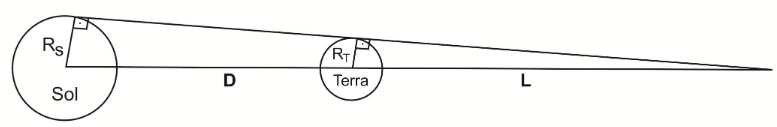
\includegraphics[scale=0.5]{img/2a.png}
            \end{figure}
            \begin{itemize}
                \item \textbf{Pergunta 2a) (0,5 ponto)} Calcule, em termos do raio da Terra ($R_T$) qual é o comprimento ($L$) da sombra  da  Terra,  mostrado  na  figura acima. Observação: $L$  é  medido  do  vértice  do  cone  de sombra até o centro da Terra.
                    \begin{itemize}
                        \item[$(\red{X})$] $L = 219,3 \cdot R_T$
                        \item[$(\quad)$] $L = 300,2 \cdot R_T$
                        \item[$(\quad)$] $L = 150 \cdot R_T$
                        \item[$(\quad)$] $L = 278,4 \cdot R_T$
                    \end{itemize}
                \item \textbf{Pergunta 2b) (0,3 ponto)} A  Lua cruza  o  cone  de  sombra  da  Terra  a uma distância $H = 60 \cdot R_T$. Calcule o raio ($d$) do cone de sombra nessa distância $H$, medido entre os centros da Terra e da Lua (não desenhada na figura), em função do raio da Terra ($R_T$).
                    \begin{figure}[H]
                        \centering
                        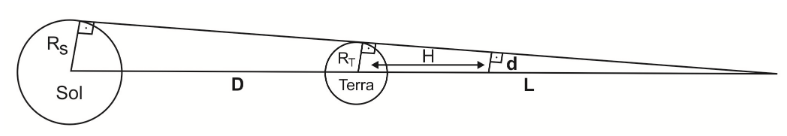
\includegraphics[scale=0.5]{img/2b.png}
                    \end{figure}
                    \begin{itemize}
                        \item[$(\red{X})$] $d = 0,73 \cdot R_T$
                        \item[$(\quad)$] $d = 1,5 \cdot R_T$
                        \item[$(\quad)$] $d = 0,25 \cdot R_T$
                        \item[$(\quad)$] $d = 2,77 \cdot R_T$
                    \end{itemize}
                \item \textbf{Pergunta 2c) (0,2 ponto)} Sabendo-se  que $R_T = 3.6 \cdot R_L$,  onde $R_L$ é o raio da Lua, calcule quantas vezes $d$ é maior do que $R_L$. Isso explica o porquê do eclipse lunar ser longo.
                    \begin{itemize}
                        \item[$(\red{X})$] $d = 2,63 \cdot R_L$
                        \item[$(\quad)$] $d = 3,14 \cdot R_L$
                        \item[$(\quad)$] $d = 1,36 \cdot R_L$
                        \item[$(\quad)$] $d = 2,15 \cdot R_L$
                    \end{itemize}
            \end{itemize}

        \item \textbf{Questão 3) (1 ponto)} Você deve ter ouvido falar dos satélites geoestacionários: aqueles que ficam sempre sobre o mesmo lugar na Terra (porque seu período para completar uma órbita é igual ao período de rotação da Terra). Esses satélites são muito úteis para transmitir sinais de televisão, rádio, telefonia, etc. \linebreak \linebreak Entretanto, para o sistema funcionar, as órbitas dos satélites estacionários devem ser todas próximas ao Equador. Logo, esses satélites não são bons para países muito ao norte ou muito ao sul. Por isso a Rússia desenvolveu um sistema diferente de satélites, chamados de Molniya. Trata-se de três satélites com órbitas bastante alongadas, como mostra a figura abaixo. \linebreak \linebreak Pelas Leis de Kepler, sabemos que a velocidade dos satélites é função da sua distância ao foco da elipse onde está a Terra. Dessa forma, próximo ao perigeu (o ponto mais próximo à Terra) o satélite vai passar rapidamente; próximo ao apogeu (o ponto mais distante da Terra), ele permanecerá por muito mais tempo. Assim, os astrônomos russos calculam a órbita para que o apogeu esteja por cima da Rússia. Além disso, eles colocam três satélites para que, a qualquer hora do dia, sempre haja pelo menos um satélite sobrevoando o território russo, para poder transmitir sinais. \linebreak \linebreak Considere o satélite Molniya da figura abaixo. Seu apogeu ($R_a$) está a $45.590 \, km$ do centro da Terra; seu perigeu ($R_p$), a $6.920 \, km$.
            \begin{figure}[H]
                \centering
                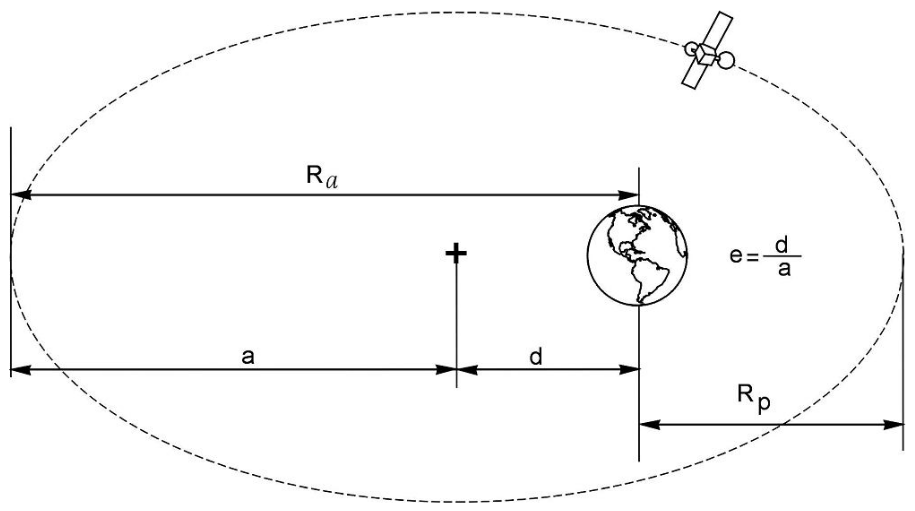
\includegraphics[scale=0.5]{img/3.png}
            \end{figure}
            \begin{itemize}
                \item \textbf{Pergunta 3a) (0,5 ponto)} Calcule o semi-eixo maior ($a$) da órbita.
                    \begin{itemize}
                        \item[$(\red{X})$] $a = 26.255 \, km$
                        \item[$(\quad)$] $a = 15.365 \, km$
                        \item[$(\quad)$] $a = 32.415 \, km$
                        \item[$(\quad)$] $a = 10.213 \, km$
                    \end{itemize}
                \item \textbf{Pergunta 3b) (0,5 ponto)} Calcule a excentricidade  ($e= \frac{d}{a}$) da órbita.
                    \begin{itemize}
                        \item[$(\red{X})$] $e = 0,74$
                        \item[$(\quad)$] $e = 0,23$
                        \item[$(\quad)$] $e = 0,95$
                        \item[$(\quad)$] $e = 1,24$
                    \end{itemize}
            \end{itemize}

        \item \textbf{Questão 4) (1 ponto)} A luminosidade (quantidade de energia emitida por unidade de tempo) é uma característica intrínseca de uma estrela, ou seja, só depende dela mesma. A estrela Betelgeuse (alfa de Órion), por exemplo, tem uma luminosidade 200 vezes maior do que Sírius, mas Sírius é a estrela mais brilhante do nosso céu noturno! O que acontece é que Sírius, apesar de não ser tão luminosa, está muitas vezes mais próxima da Terra que Betelgeuse. O mesmo ocorre, de forma muito mais acentuada, com o nosso Sol. Ele tem uma luminosidade ainda menor que a de Sírius, mas está muito, mas muito mais próximo mesmo da Terra, e por isso é praticamente a única fonte de energia do nosso planeta. Como calcular isso? É simples: a luz emitida por uma estrela sai de sua superfície igualmente em todas as direções. Ou seja, a energia que sai da estrela vai se espalhando igualmente em todas as direções pelo espaço, conforme vai se afastando da estrela. Assim, não importa se estamos vendo a estrela de um lado ou de outro, importa apenas a distância. E você já deve ter aprendido que o lugar geométrico de todos os pontos a uma mesma distância de outro ponto desenha no espaço uma superfície esférica, uma casca esférica. Suponha então que estamos em um lugar, a uma distância qualquer (que podemos representar pela letra d, como na fórmula abaixo) de uma estrela que tenha uma luminosidade qualquer (representada aqui pela letra ele maiúscula $L$, na fórmula abaixo). Queremos saber quanta energia chega em uma unidade de área deste lugar, por unidade de tempo. Quando a luz da estrela chegar neste lugar, ela terá se espalhado por toda a região que esteja à mesma distância da estrela, ou seja, pela superfície de uma suposta esfera de raio $d$, que tem área $4 \cdot \pi \cdot d^2$. Assim, a energia que chega por unidade de tempo, por unidade de área, a essa distância é chamada de fluxo ($F$) e é dada por $F = \frac{L}{4 \pi d^2}$. Assim, podemos dizer que, embora Betelgeuse seja mais luminosa, Sírius está mais perto, e então o fluxo de Sírius medido na Terra é maior -- o que a faz aparecer mais brilhante do que Betelgeuse.
            \begin{itemize}
                \item \textbf{Pergunta 4a) (0,5 ponto)} Você deve imaginar que a luminosidade, sendo uma medida de energia por tempo, pode ser medida em unidades de potência, isto é, energia por tempo. Vamos adotar aqui, como unidade de potência, o Watt, que é a unidade do sistema internacional de unidades (SI). Um Watt representa um Joule (a unidade de energia do SI) por segundo (Watt = Joule/segundo). A luminosidade do Sol ($L_S$) é de $4 \cdot 10^{26}$ Watts. Calcule seu fluxo aqui na Terra ($F_{S-T}$). Em outras palavras, quanta energia solar chega na Terra por segundo, por metro quadrado? Dados: distância Terra-Sol = 150 milhões de quilômetros = $15 \cdot 10^{10} \, m$; use $\pi = 3$.
                    \begin{itemize}
                        \item[$(\red{X})$] $F_{S-T} = 1,5·10^3 \, \frac{W}{m^2}$
                        \item[$(\quad)$] $F_{S-T} = 3,2·10^3 \, \frac{W}{m^2}$
                        \item[$(\quad)$] $F_{S-T} = 1,5·10^4 \, \frac{W}{m^2}$
                        \item[$(\quad)$] $F_{S-T} = 3,2·10^4 \, \frac{W}{m^2}$
                    \end{itemize}
                \item \textbf{Pergunta 4b (0,5 ponto)} Se medirmos, de fato, o fluxo na superfície terrestre ($F_{S-T}$), o valor será significativamente menor. Por quê?
                    \begin{itemize}
                        \item[$(\red{X})$] A atmosfera atua como um poderoso filtro da radiação solar.
                        \item[$(\quad)$] Parte da radiação solar é perdida ao atravessar o vácuo entre o Sol e a Terra.
                        \item[$(\quad)$] Na prática, o Sol não emite toda sua luminosidade.
                        \item[$(\quad)$] Nossos aparelhos não são capazes de medir o valor total desse fluxo.
                    \end{itemize}
            \end{itemize}

        \item \textbf{Questão 6) (1 ponto)} As estrelas se formam a partir da fragmentação, seguida da condensação, de nuvens de gás (principalmente Hidrogênio) e poeira muito pouco densas presentes nas galáxias. E isto acontece exatamente porque esta matéria, mesmo muito difusa, se atrai segundo a Lei da Gravitação Universal. À medida que a assim chamada nuvem proto-estelar (pois ainda não é uma estrela) se contrai, sob a influência de sua própria gravitação, a sua temperatura aumenta devido à energia liberada pela contração. É como se a nuvem caindo sobre ela mesma liberasse a energia da queda Neste estágio a proto-estrela emite radiação no infra-vermelho. Isto é, ainda não podemos ver a estrela, pois ela está emitindo energia em um comprimento de onda menor do que o comprimento da cor vermelha. Quando a temperatura central da nuvem atinge cerca de dez milhões de graus os núcleos de Hidrogênio (H) começam a sofrer fusão se transformando em núcleos de Hélio (He) na proporção de 4 H para 1 He. A energia obtida com a conversão de H em Hélio (He) é suficiente para suprir as necessidades da estrela. A contração cessa, pois agora existe uma fonte de energia térmica que se contrapõe ao colapso gravitacional, e a estrela atinge uma situação de equilíbrio. Assim, os núcleos das estrelas como o Sol, que queimam Hidrogênio são imensos reatores termo-nucleares, isto é, produzem energia na forma de calor a partir de fusão nuclear. A estrela se mantém estável até que o H do seu núcleo seja consumido, mas isso leva muito tempo, o qual representa aproximadamente $90\%$ da vida da estrela. É nesta fase de equilíbrio, conhecida também como sequência principal, em que o nosso Sol se encontra. A “queima” de Hidrogênio em Hélio produz energia em virtude da conversão de uma pequena quantidade de massa dos átomos de Hidrogênio em energia segundo a famosa fórmula de Albert Einstein de que uma dada quantidade de massa pode ser convertida inteiramente em energia tendo como constante de proporcionalidade o quadrado da velocidade da luz, $E = mc^2$. Essa constante de proporcionalidade confere uma altíssima produção de energia mesmo para quantidades muito pequenas de massa, pois a velocidade da luz é da ordem de $300.000 \, km/s$. Assim, o átomo de He tem uma massa apenas um pouco menor do que a de 4 H. É assim que o Sol vem produzindo energia já há 4,5 bilhões de anos. \linebreak \linebreak Dados:\linebreak$>$ Um grama de matéria totalmente convertida em energia produz 90 trilhões de Joules ($9 \cdot 10^{13} \, \frac{kgm^2}{s^2}$).\linebreak$>$ Sabemos com certeza que o Sol converte aproximadamente 600 milhões de toneladas ($6 \cdot 10^{11} \, kg$) de Hidrogênio em Hélio por segundo e que apenas $1\%$ da massa do Hidrogênio é de fato “queimada” na produção de He.\linebreak$>$ Um grama de Hidrogênio contém aproximadamente $6 \cdot 10^{23}$ átomos.
            \begin{itemize}
                \item \textbf{Pergunta 6a) (0,5 ponto)} Calcule a quantidade total de energia produzida pelo Sol a cada segundo.
                    \begin{itemize}
                        \item[$(\red{X})$] $5,4 \cdot 10^{26} \, J$
                        \item[$(\quad)$] $5,4 \cdot 10^{27} \, J$
                        \item[$(\quad)$] $2,7 \cdot 10^{25} \, J$
                        \item[$(\quad)$] $2,7 \cdot 10^{26} \, J$
                    \end{itemize}
                \item \textbf{Pergunta 6b) (0,5 ponto)} Calcule quantos átomos de Hélio são produzidos pelo Sol a cada segundo.
                    \begin{itemize}
                        \item[$(\red{X})$] $9 \cdot 10^{37}$ átomos
                        \item[$(\quad)$] $9 \cdot 10^{35}$ átomos
                        \item[$(\quad)$] $5 \cdot 10^{34}$ átomos
                        \item[$(\quad)$] $5 \cdot 10^{36}$ átomos
                    \end{itemize}
            \end{itemize}
        
        \item \textbf{Questão 7) (1 ponto)}
            \begin{itemize}
                \item \textbf{Pergunta 7a) (0,3 ponto)} Considere que o Sol atinge o Zênite de um lugar num solstício. Em qual região esse lugar se situa e qual é a estação do ano nesse hemisfério?
                    \begin{itemize}
                        \item[$(\red{X})$] Sobre qualquer um dos trópicos; verão.
                        \item[$(\quad)$] Sobre qualquer um dos trópicos; inverno.
                        \item[$(\quad)$] Entre os trópicos; verão.
                        \item[$(\quad)$] Entre os trópicos; inverno.
                    \end{itemize}
                \item \textbf{Pergunta 7b) (0,3 ponto)} O Sol, no ponto diurno mais alto no céu de um determinado lugar, nunca atinge o Zênite. Em que região esse lugar se encontra?
                    \begin{itemize}
                        \item[$(\red{X})$] Entre um trópico e o respectivo polo.
                        \item[$(\quad)$] Entre os trópicos.
                        \item[$(\quad)$] Sobre qualquer um dos trópicos.
                        \item[$(\quad)$] Sobre o Equador.
                    \end{itemize}
                \item \textbf{Pergunta 7c) (0,4 ponto)} A maior altura que o Sol atinge em um lugar é igual à inclinação do eixo de rotação da Terra com relação à perpendicular ao plano de translação. Que lugar da Terra é esse e quando isso ocorre?
                    \begin{itemize}
                        \item[$(\red{X})$] Sobre qualquer um dos polos.
                        \item[$(\quad)$] Sobre qualquer um dos trópicos.
                        \item[$(\quad)$] Sobre o Equador.
                        \item[$(\quad)$] Não há informações suficientes para responder esta pergunta.
                    \end{itemize}
            \end{itemize}
    \end{itemize} \end{flushleft}

    \begin{flushright}
		\begin{large}
			Bons estudos!
		\end{large}
	\end{flushright}
\end{document}